\subsection{IFIT Subcellular Localisation During Interferon Induction and RSV Infection} \label{subsec:IFIT Subcellular Localisation During Interferon Induction and RSV Infection}
introduction for why we wanted to look at colocalisation of ifit durng infection and elsevere

To investigate this, we seeded A549, MDBK, and later BEAS2B cell lines on a 13 mm diameter glass coverslip in a 24-well plate in a initial concentration on 100,000 cells per well as described in Section \ref{sec:Cell Culture}. 24 hours post seeding these cells were either mock infected; treated with either human or bovine interferon alpha at concentrations of 1,000 international units per mL for the former or 5 ng/mL (these concentrations correspond to each other); or infected with either human or bovine wild-type RSV at MOI of 1. After 24 hours the samples were fixed with paraformaldehyde and prepared as described in Section \ref{sec:Confocal Microscopy} for the subsequent confocal microscopy analysis.

Figure \ref{fig:The Changes in Subcellular Localisation of Human IFITs in A549 Cells Subjected to hIFNa or hRSV} ... 

hIFIT1 is cytoplasmic and nuclearly excluded in a basal state. Interestingly, hIFNa stimulation does not alter this localisation pattern, neither the abundance of IFIT1 as detected by the intensity of the signal. During infection IFIT1 stays cytoplasmic and excluded from nucleus with a possible colocalisation with N, on the outside of the IB structure. The intencity of staining is increased, especially in uninfected cells, suggesting hypothesis from chapter 1 is correct. IFIT2A antibody shows hIFIT2 to be located in cytoplasmicly diffused but nuclearly excluded vesicular pattern, for both basal pattern and IFNa induced pattern. The intensity between these two conditions appear to be equal. During hRSV infection, the overal intensity seems to decrease. The subcellular localisation also changes into a phenotype with less vesicules and inclusions inside the RSV IB structures. IFIT2B antibody on the other hand detects IFIT2 to be granular and cytoplasmic, while also showing to be excluded from the nucleus. Like with IFIT2A antibody, the intensity and localisation phenotype between mock and IFNa treated cells is equal. During hRSV onfection, this antibody detect IFIT2 to be excluded from both the nucleus and the inclusion body, while retaining vesicular cytoplasmic stain. IFIT3 appears to be cytoplasmic with nuclear exclusion under basal conditions. After IFNa treatment we can observe increase in the staining intensity and signs of IFIT3 nuclear translocation. During hRV infection IFIT3 seems to be evenly diffused throught the whole cell, including the RSV inclusion body and the nucleus. The intesity of staining during infection appears similar between IFNa treated and hRSV infected cells. IFIT5 is also cytoplasmically located under basal conditions while being excluded rom the nucleus. During IFNa treatment the phenotype and the intensity of the staining remain the same. Dyring hRSV infection, we can see uninfected cells dyspaing increased IFIT5 levels. With regards to the staining pattern, it remains cytoplasmic and excluded from both nucleus and RSV IB.

\begin{figure}
    \centering
    \includegraphics[width=1\linewidth]{08. Chapter 3/Figs/01. Localisation introduction/07. a549 merges.pdf}
    \caption[The Changes in Subcellular Localisation of Human IFITs in A549 Cells Subjected to hIFN\(\alpha\) or hRSV.]{\textbf{The Changes in Subcellular Localisation of Human IFITs in A549 Cells Subjected to hIFN\(\alpha\) or hRSV.} A549 cell were either mock treated, or treated with 1000 IU/mL of hIFN\(\alpha\) for 24 hours, or were infected with hRSV MOI 1 for 24 hours. Cells were fixed, and stained with DAPI (nuclei detection; yellow), anti-RSV N antibody (cyan), or with antibodies against IFIT proteins (magenta). Two antibodies against IFIT2 were used, termed IFIT2A and IFIT2B. Insets with magnified selections were created from infected images to more easily convey the underlying subcellular localisations.}
    \label{fig:The Changes in Subcellular Localisation of Human IFITs in A549 Cells Subjected to hIFNa or hRSV}
\end{figure}


Figure \ref{fig:The Changes in Subcellular Localisation of Bovine IFITs in MDBK Cells Subjected to bIFNa or bRSV} ...

In MDBK cells, bIFIT1 under basal conditions is located cytoplasmicly with nuclear exclusion. In some cells we can see vesicules located throught the cells. Upon bIFNa stimulation we can see that the subcellular localisation remains unchanged. What changes is the overall intensity of staining. Samples infected with bRSV show cytoplasmic staining with nuclear and IB exclusion, without any ovious vesicules. Surrounding non infected cells dysplay increased IFIT1 signal, while infected cells show staioning intensity lower than what we observed with interferon stimulated cells. IFIT2A antibody detects bIFIT2 to be predonimantly cytoplasmic with concentrations in a proximity to nucleus which resemble the endoplasmic reticulum. This signal is also excluded from the nucleus. In interferon treaded cells, the overal pattern apperas to be the same with the expetion of decreased staining intensity and decreased size of nucleraly proximal condensations. During bRSV infection we see results identical to wat was observed in A549 cell line. The cytoplasmic signal is greatly reduced and instead IFIT2 either colocalises with RSV N on the baundry of the IB, or concentrates inside the inclusion bodies as a inclusion. IFIT2B on the other hand shows bIFIT2 to be cytoplamic with vesicules present spread through the cytoplasm and nucleus under basal conditions. Unfortunately we lack the cells treated with bIFNa that were stained with IFIT2B antibody. During bRSV infection, this antibldy shows bIFIT2 to have the same localisation and intensity as what was observed in mock cells. It also shows IFIT2 to be excluded from the IB structure. bIFIT3 appears to be localised in vesicules with cytoplasmic and nuclear localisation in both mock and bIFNa treated cells. The intensity signal appears to be slightly stronger in the interferon treated samples. During bRSV infection IFIT3 subcellular localisation changes drasticaly. It is barely detectable in cytoplasm and nucleus with the expeption of strong intra inclusion body inclusions. There also appears to be vesicles inside the inclusion that resembles the IBAGs. Last but not least, bIFIT5 shows cytoplasmic localisation with vesicles diffused through the cytoplasm, weak nuclear staining and inclusion within nuclei, most probaly colocalising with the nucleololi. In the samples treated with bIFNa, we cna see that although the pattern of subcellular localisation stays the same, the intensity is increased, especially in the nucleus. Finally, in the cells infected with the bRSV, we can observe nuclear exclusion with inclusion within the nucleoi; cytoplasmic staining with no obvious either colocalisation nor exclusion with RSV IBs. We can also see the cytoplasmic vesicles observed previously, although only in non-infected cells. The intensity of the staining resembles the one of mock treated cells.

\begin{figure}
    \centering
    \includegraphics[width=1\linewidth]{08. Chapter 3/Figs/01. Localisation introduction/09. mdbk-merges-test.pdf}
    \caption[The Changes in Subcellular Localisation of Bovine IFITs in MDBK Cells Subjected to bIFN\(\alpha\) or bRSV.]{\textbf{The Changes in Subcellular Localisation of Bovine IFITs in MDBK Cells Subjected to bIFN\(\alpha\) or bRSV.} MDBK cell were either mock treated, or treated with 5 ng/mL of bIFN\(\alpha\) for 24 hours, or were infected with bRSV MOI 1 for 24 hours. Cells were fixed, and stained with DAPI (nuclei detection; yellow), anti-RSV N antibody (cyan), or with antibodies against IFIT proteins (magenta). Two antibodies against IFIT2 were used, termed IFIT2A and IFIT2B. Insets with magnified selections were created from infected images to more easily convey the underlying subcellular localisations.}
    \label{fig:The Changes in Subcellular Localisation of Bovine IFITs in MDBK Cells Subjected to bIFNa or bRSV}
\end{figure}

Puting both results together and linking it to the massive analysis ...

Seeing the potentially intersting results with IFIT colocalisation with RSV IBs, we systematically analysed 1727 IB sizes and their underlying interaction phenotype with the different IFIT proteins. We categorised the phenotypes solely based on the IFIT staining, but in the area of the image where a presence of inclusion body was confirmed by viral protein staining. Based on our observations, we decided to categorise the phenotypes in a following manner: \textbf{Diffusion} phenotype would be assigned if the IFIT signal would be equally spread through the area if interest; \textbf{Exclusion} phenotype, which would be assigned by a obvious, partial or full, decrease in signal within the boundry of IB; \textbf{Edge exclusion} phenotype would be assigned if the IFIT signal would be equally spread through the area if interest with the exeption of IB boundry, from which it would be excluded; \textbf{Inclusion} phenotype would be assignes if there was obvious increase in the IFIT signal within the boundry of IB; and \textbf{Colocalisation} phenotype, which would be assigned if the IFIT signal would be equally spread through the area if interest with the exeption of increased signal in the IB boundry. These main phenotypes were also simetimes supplemented by either their interaction, or the presence of spots within the IB boundry. For the former, a very common occurance was colocalisation accompanied by exclusion. This was when there was an obvious increase on the IB boundry compared to the surrounding signal, while also a marked decrease of signal from within the region of interest was present. For the latter, these spots were termed IBAGs, as we speculate that these structures could be inclusion body associated granules.

about setting gains menaing two images dont have the same intensities but signal is real. extending the useful range etc..  we cared about the observed phenotype. bilinear interpretation etc ... put the Figure \ref{fig:Inclusion Bodies Within RSV Infected Cells: Zoom Sequence} as an example of analysis and final images ... 

\begin{figure}
    \centering
    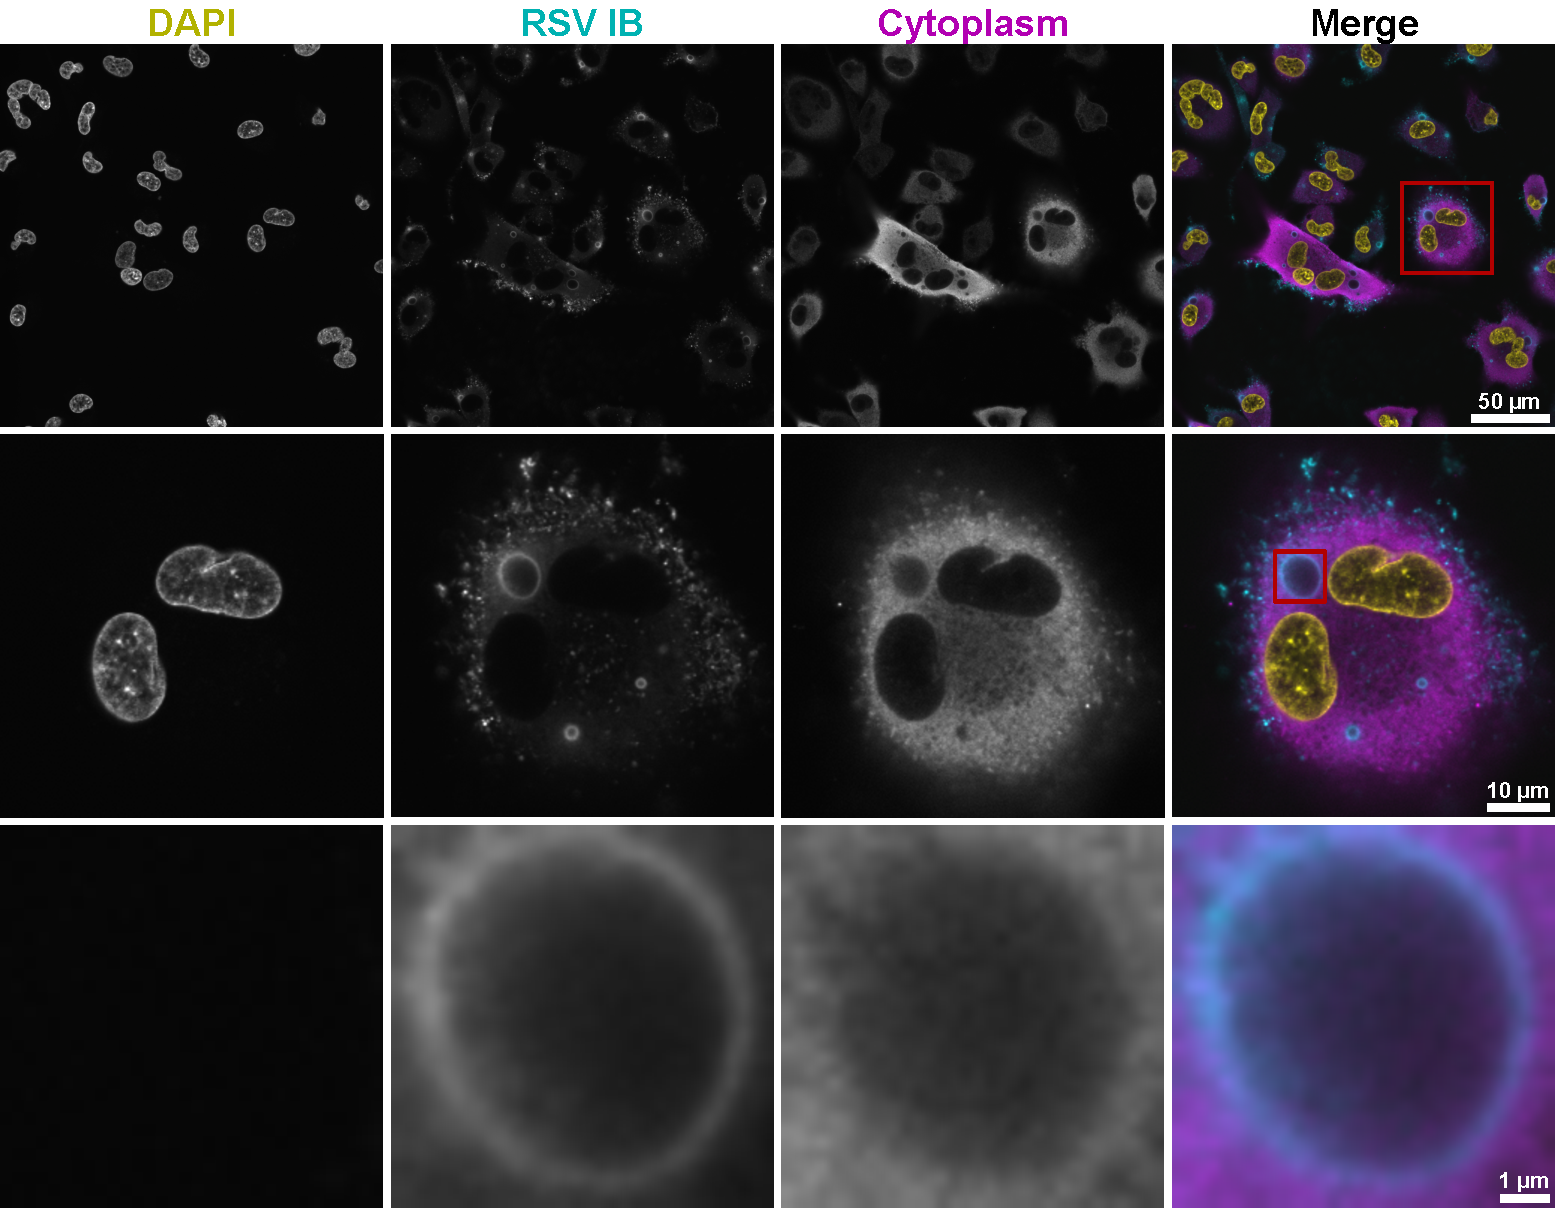
\includegraphics[width=1\linewidth]{08. Chapter 3/Figs/01. Localisation introduction/01. IB-zooms.pdf}
    \caption[Inclusion Bodies Within RSV Infected Cells: Zoom Sequence.]{\textbf{Inclusion Bodies Within RSV Infected Cells: Zoom Sequence.} A represerenative image of RSV infected cells detected using confocal microscopy. Cellular nuclei were stained with DAPI and are shown in yellow; RSV inclusion bodies are shown in cyan; and the cytoplasm is shown in magenta. Figure highlights a zoom sequence from a population of cells, into a single syncytia view, with lastly focusing at one individual inclusion body.}
    \label{fig:Inclusion Bodies Within RSV Infected Cells: Zoom Sequence}
\end{figure}

% introduction to ib stuff from my study
write about ib size statistics from my analysis

\begin{figure}
    \begin{subfigure}{0.495\textwidth}
        \caption{}
        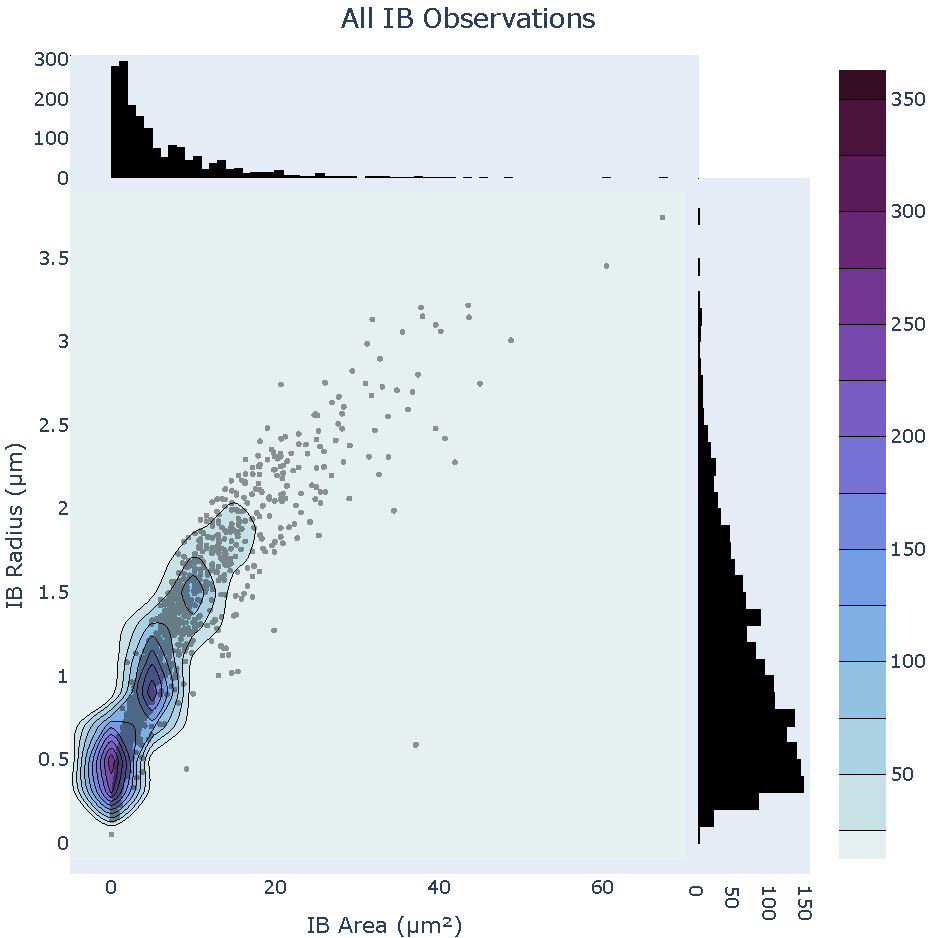
\includegraphics[width=\textwidth]{08. Chapter 3/Figs/01. Localisation introduction/02. heatmap_all.pdf} 
    \end{subfigure}
    \hfill
    \begin{subfigure}{0.495\textwidth}
        \caption{}
        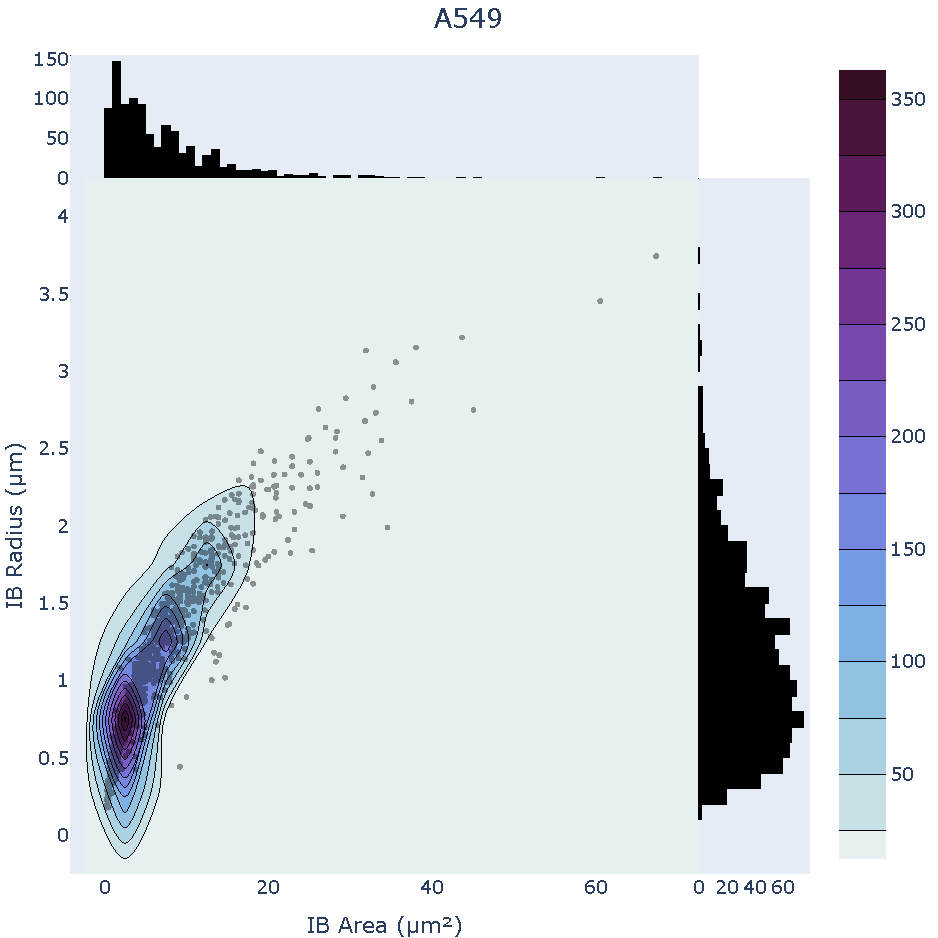
\includegraphics[width=\textwidth]{08. Chapter 3/Figs/01. Localisation introduction/03. heatmap_a549.pdf}
    \end{subfigure}

    \medskip
    \begin{subfigure}{0.495\textwidth}
        \caption{}
        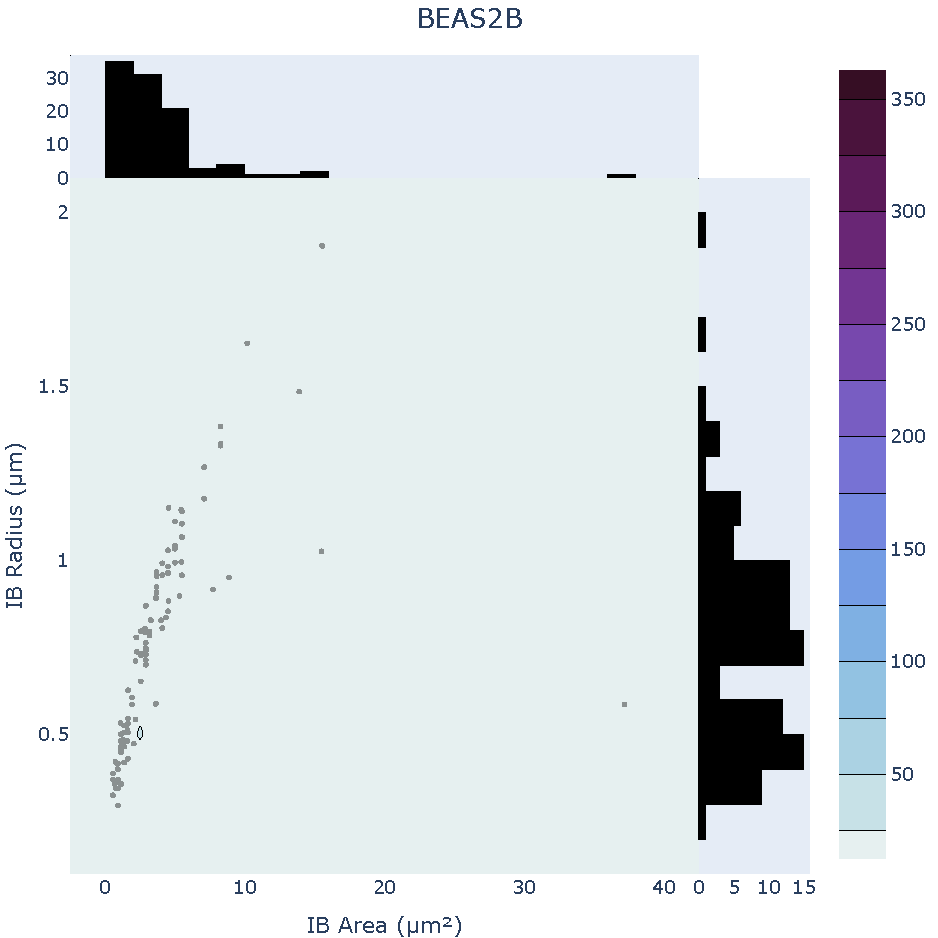
\includegraphics[width=\textwidth]{08. Chapter 3/Figs/01. Localisation introduction/04. heatmap_beas2b.pdf} 
    \end{subfigure}
    \hfill
    \begin{subfigure}{0.495\textwidth}
        \caption{}
        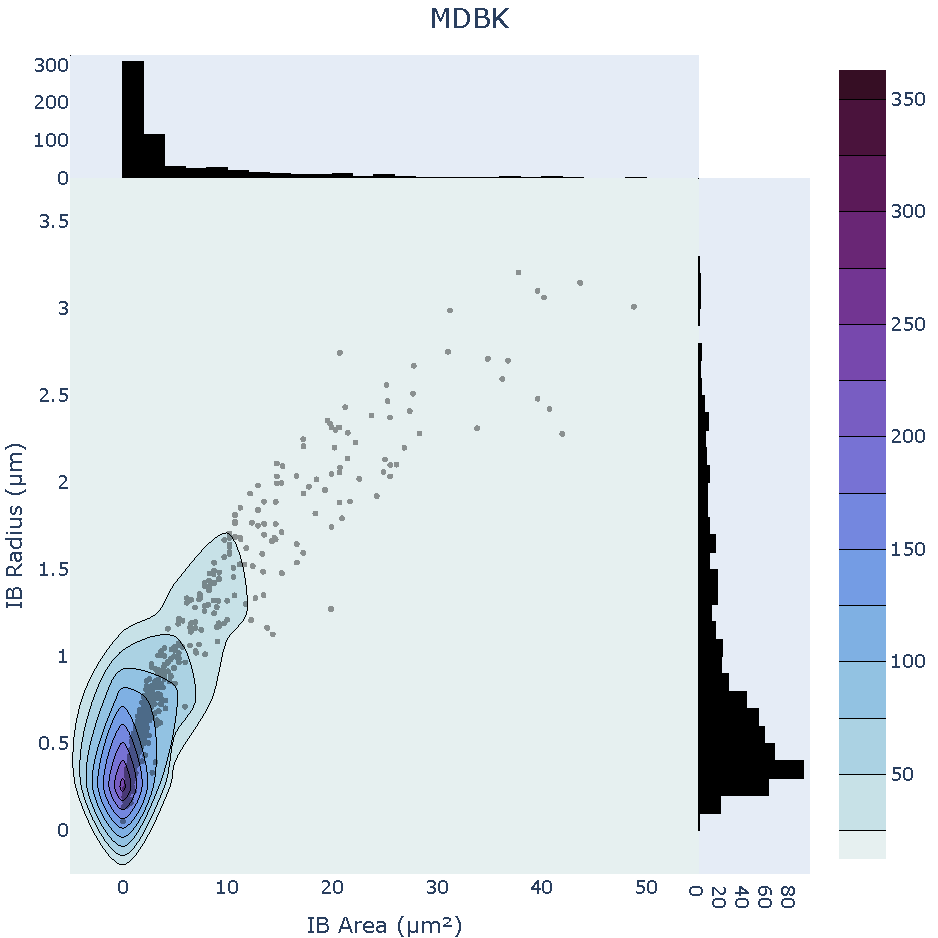
\includegraphics[width=\textwidth]{08. Chapter 3/Figs/01. Localisation introduction/05. heatmap_mdbk.pdf} 
    \end{subfigure}
    
    \caption[Size Characterization of Inclusion Bodies Across Different Cell Lines.]{\textbf{Size Characterization of Inclusion Bodies Across Different Cell Lines.} This figure presents the relationship between the measured area (\(\mu m^2\)) and diameter (\(\mu m\)) of individual inclusion bodies (IBs) as observed within the scope of this study. Additionally, the figure includes distinct population distributions depicted alongside the plots, representing (a) the aggregate of 1727 observations of IBs across all individual cell lines, (b) 1008 observations from the A549 cell line, (c) 99 observations from the BEAS2B cell line, and (d) 620 observations from the MDBK cell line. Contour plots are incorporated to elucidate the underlying density of individual IBs within the plots.}
    \label{fig:Size Characterization of Inclusion Bodies Across Different Cell Lines}  
\end{figure}

decribe the size data

there is a clear difference in sizes detected in our study
compare to published and fj thesis
mdbk has more small ibs
each cell line seems to have also unusally large ibs


\begin{figure}
    \centering
    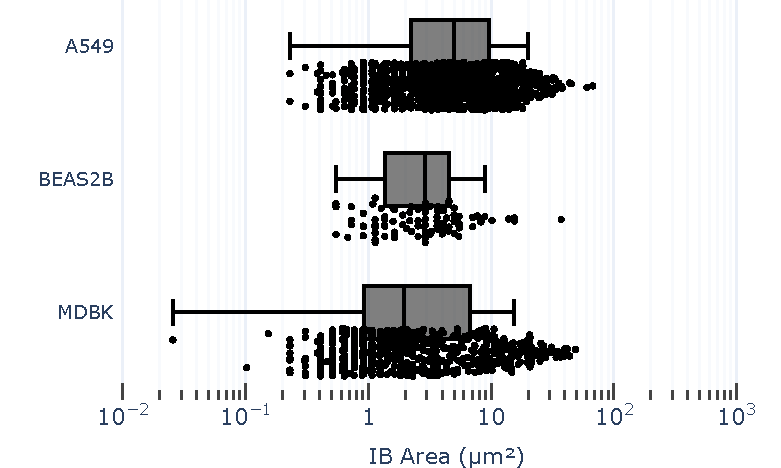
\includegraphics[width=1\linewidth]{08. Chapter 3/Figs/01. Localisation introduction/06. box-infection.pdf}
    \caption[boxplot of ib sizes per cell line.]{\textbf{boxplot of ib sizes per cell line.} this is the data from above but only area, to be able to compare it later}
    \label{fig:boxplot of ib sizes per cell line}
\end{figure}

write about the distributions of area between the different cell lines

5, 3, 2 areas